\documentclass[twoside]{article}
\usepackage{aistats2015}
\usepackage{graphicx}
\usepackage{pgfplots}
\usepackage{float}
\usepackage{subfig}
\usepackage{hyperref}
\usepackage{natbib}
\usepackage{amsmath}

\bibpunct{[}{]}{;}{n}{,}{,}

\newlength\figureheight \newlength\figurewidth % ?

\begin{document}

\twocolumn[
\aistatstitle{Learning to Control Kilobots with a Flashlight}
\aistatsauthor{Alexander Hendrich \And Daniel Kauth \And Gregor Gebhardt}
\aistatsaddress{TU Darmstadt \And TU Darmstadt \And TU Darmstadt}]

\begin{abstract}
The recently emerged kilobots provide lots of new applications for swarm
intelligence and collective behavior algorithms. By applying a light following
behavior called \emph{Phototaxis} to the kilobots, they provide an easy method
to move and control large quantities at the same time. By interacting with the
lightsource(s) (switching them on/off or moving a single light source) a human
can control a kilobot swarm to fulfill certain tasks, for example pushing an
object through a maze\cite{kilobotMaze}. In this project we want to learn to
control the light to achieve this behavior.
\end{abstract}

\section{INTRODUCTION}

Our task is to learn to push an object through a maze with a swarm of kilobots
by moving a single light source. Because this task is quite complex and
difficult to learn, we split it up into two separate problems with two separate
policies.

The first problem is to find an optimal path through the labyrinth. The policy
should return a movement direction for each possible object position. By
constantly following these movements, the object should reach the goal position
independent of its starting position.

Because we cannot directly control the object's movement we need a method to
interact with the light source, so that the kilobots push the object in the
desired direction. This will be the focus of the second problem. The policy
should return a new light position depending on the output of the first policy
(the desired movement direction of the object) and the relative position of the
kilobots towards the object.

\begin{figure}[!htb]
    \centering
    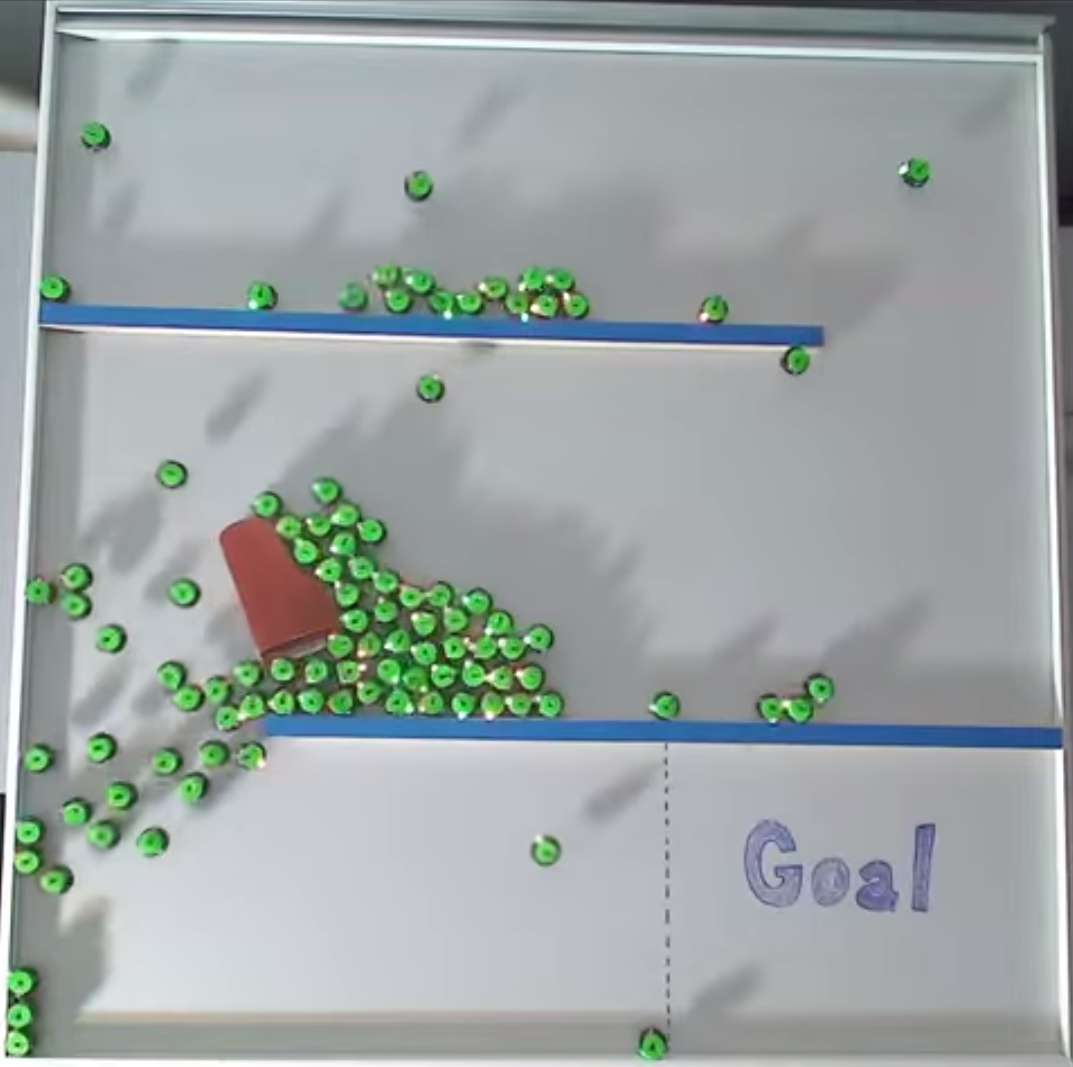
\includegraphics[width=0.8\linewidth]{figures/inspiration.png}
    \caption{Kilobots pushing a small object through a maze by human controlled
        light sources}
\end{figure}

\section{PRELIMINARIES}
In the following sections we introduce our used materials
(kilobots\cite{kilobot}) and methods (Actor Critic Relative Entropy Policy
Search)\cite{acreps}.

\subsection{Kilobots}
Kilobots\cite{kilobot} are open-source, low cost robots specially designed to
explore collective algorithms and decentralized cooperation. With previous
robots these methods could only be tested in a simulator or in small quantities
of robots because acquiring and controlling hundreds or even thousands of them
is very cost-intensive, time consuming and complex. To eliminate this issue
Harvard University developed Kilobots. Each robot is made with only 14\$ worth
of parts and large collectives can easily be controlled by a single user.

The low cost however results in limited capabilities of each individual robot.
For example, the kilobot doesn't use complex steering or wheels for locomotion.
Instead it stands on three solid legs and moves by activating two small
vibrating motors placed on each side of the kilobot. This form of movement only
allows for very low movement speeds of up to 1cm per second and can only be
performed on special surfaces (e.g. glass).

To communicate with each other, each kilobot has an infrared transmitter and
receiver on the bottom. Messages are passed by emitting infrared light onto the
reflecting glass and can be received by another kilobot up to 7-10cm away
(radius of each kilobot is 3.3cm). By measuring the received signal strength,
the kilobots are capable of estimating their distances to each other.

The kilobot also possesses an ambient light sensor to determine the light
intensity at its current location. Depending on the current and previously
measured light intensity the robot alternates between left and right turns to
move towards the light source. This behavior is called \emph{Phototaxis} and is
used to control a whole swarm of robots at once. While performing left or right
turns the robot only activates one of its two motors and the robot doesn't move
in a straight line, which further reduces its movement speed.

\begin{figure}[!htb]
    \centering
    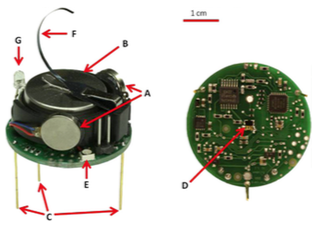
\includegraphics[width=0.9\linewidth]{figures/kilobot.png}
    \caption{Isometric (left) and bottom (right) views of a Kilobot. Some key
        features are: (A) vibration motors, (B) lithium-ion battery, (C) rigid
        supporting legs, (D) infrared transmitter/receiver, (E) three-color
        (RGB) LED, (F) charging tab, and (G) ambient light sensor. Note the 1 cm
        line for scale.\cite{kilobot}}
\end{figure}

\subsection{Actor Critic Relative Entropy Policy Search}
\emph{Actor critic relative entropy policy search} (AC-REPS) as introduced by
\cite{acreps} is a method for policy improvement based on \emph{relative entropy
policy search} (REPS) \cite{reps} which allows for model-free learning with
non-parametric continous policies and random exploration. It consists of the
following three steps:

\subsubsection{Estimating the Q-Function}
During the simulation we generate sample in the form $(s_i, a_i, r_i, s'_i)$,
where we start in state $s_i$, take action $a_i$ to get to state $s'_i$ and
get reward $r_i$. We also define a feature-based Q-function as $Q(s, a) =
\phi(s,a)^T \theta$ with feature function $\phi(s,a)$ and parameter vector
$\theta$. Details of our state and action representations and rewards and
features we used are discussed in section TODO.

To estimate $\theta$ we use \emph{Least-squares temporal difference
learning} (LSTD) with $L_{22}-Regularization$\cite{lstdRegularization} as
follows:

With $n$ being the number of sample and $k$ being the number of features
we define the two feature matrices $\Phi$ and $\Phi'$ (size $n\times k$)
$$
\Phi = \left(
\begin{array}{c}
    \phi(s_1,a_1)^T \\
    \phi(s_2,a_2)^T \\
    \dots \\
    \phi(s_n,a_n^T)
\end{array} \right), \;
\Phi' = \left(
\begin{array}{c}
    \mathbf{E}_{\pi(a_1'|s_1')} [\phi(s_1', a_1') | s_1']^T \\
    \mathbf{E}_{\pi(a_2'|s_2')} [\phi(s_2', a_2') | s_2']^T \\
    \dots \\
    \mathbf{E}_{\pi(a_n'|s_n')} [\phi(s_n', a_n') | s_n']^T \\
\end{array} \right)
$$
and the reward vector
$$
R = \left(
\begin{array}{c}
    r(s_1) \\
    r(s_2) \\
    \dots \\
    r(s_n)
\end{array} \right).
$$
For $\Phi'$ we estimate the expected value
$$
\mathbf{E}_{\pi(a_i'|s_i')} [\phi(s_i', a_i') | s_i']
$$
by taking the average over $m$ samples $a_i' \sim \pi(a_i'|s_i')$, where $\pi$
is our current policy.

Using the derivations of \cite{lspi} and \cite{lstdRegularization} we can easily
compute $\theta$ as
$$
\theta = (X^TX+\beta'I)^{-1}X^Ty
$$
with
$$X = C(A+\beta I) \qquad y=Cb$$
$$A = \Phi^T(\phi-\gamma \Phi') \qquad b=\Phi^T R$$
$$C = \Phi(\Phi^T\Phi+\beta I)^{-1},$$
where $\beta$ and $\beta'$ are regularization parameters for the projection and
fixed-point step which make the estimation numerically more stable and improve
noise tolerance.

\subsubsection{Actor Critic REPS}
In this step we find a new policy $\pi'$ which optimizes the expected Q-value
as given by our estimated Q-function, but has a limited Kullback-Leibner (KL)
distance to the old policy $\pi$.

To achieve this we optimize over the joint state action distribution
$p(s,a) = p(s) \pi'(s, a)$ and require that the estimated state distribution
$p(s)$ is the same as in the given state sample distribution $\mu(s)$.
This is implemented by matching feature averages of $p(s)$ and $\mu(s)$ and
leads to the following optimization problem:
\begin{align*}
    & \max_p \int p(s, a)Q(s, a)\:ds\:da\:, \\
    & \text{s.t. } \text{KL}(p(s, a) || \mu(s)\pi(a|s)) \leq \epsilon,\\
    & \int p(s)\phi(s)\:ds = \hat{\phi}, \int p(s, a)\:ds\:da = 1,
\end{align*}
where $\hat{\phi} = \int p(s) \phi(s)\:ds$ is the average feature vector of all
state samples, $\phi(s)$ is another feature function and $\epsilon$ is the
maximum allowed distance between the old and new policies.

This problem can be solved using Lagrangian multipliers and has the solution
$$
p(s)\pi'(a|s) \propto \mu(s) \pi(a|s) \exp\left(\frac{Q(s,a) - V(s)}{\eta}\right),
$$
where $V(s) = v^T \phi(s)$ and $\eta$ and $v$ are Lagrangian multipliers which
can be obtained by minimizing the dual function on the samples using standard
gradient methods.

\subsubsection{Obtaining a new Policy}
The previous step only gives us desired probabilities
$p(s_i, a_i) = p(s_i) \pi'(a_i|s_i)$ for our samples so in this step we need
to generalize these by fitting a new policy $\bar{\pi}$.

This is done by minimizing the KL divergence between $\pi'$ and our new policy
$\bar{\pi}$ which is equivalent to computing a weighted maximum likelihood
estimate with sample weights
$$ w_i = \exp\left(\frac{Q(s_i, a_i) - V(s_i)}{\eta}\right). $$

In this paper we use a weighted Gaussian Process (GP) to obtain our new policy
$\bar{\pi}$ by estimating action $a_i$ for state $s_i$ with weight $w_i$. We
also use the sparse version of the GP to reduce computation time.

This choice of weights will reproduce actions wich lead to a higher reward with
higher probability but will also choose suboptimal actions with some
probability, because our new policy can not be too far away in terms of KL
divergence from the old policy and we start with a random policy. This achieves
a tradeoff between exploration and exploitation.

TODO citation / explain Sparse GP?

\section{LEARNING PROCESS}

Our learning process is implemented in Python and uses a simple kilobot
simulator (see \autoref{sec:simulator}) written by us to generate samples.

\subsection{Maze Solving Policy}
This policy tells us where the object should move given the current object
position and solves the maze (\autoref{fig:simulator}) in this way.

Because this policy is relatively easy to learn and there are specialized maze
solvers which can easily compute an optimal path through any maze we did not
learn this policy and instead focused on the second one, which is much more
interesting. Therefore we manually specified this policy by providing a number
of waypoints the object should pass and giving the next waypoint as the target
position. Once we reach a waypoint we move one to next one.

In our experiments this simple policy is sufficient to move different objects
through a simple maze using our object movement policy. For this reason we will
only discuss the object moving policy in the following sections.

TODO dont learn first part because already done in first paper?
TODO use maze solver or just points list?

\subsection{Simulator}
\label{sec:simulator}

\newcommand\nkb{\#\mathit{kb}}
\newcommand\nep{\#\mathit{ep}}
\newcommand\nst{\#\mathit{st}}

To simulate the kilobots and collect samples for the object movement policy we
wrote our own simple kilobot simulator (\autoref{fig:simulator}) in Python based
on the 2D physics engine pybox2d\cite{pybox2d}. This allows us to simulate
collisions between kilobots and other kilobots, the object and walls.

When requesting new samples from the simulator we specify the current policy
$\pi$ which will be used to generate these sampels as well as the sampling
parameters such as the shape of the object, the number of kilobots $\nkb$, the
number of episodes $\nep$ and the number of steps per episode $\nst$.

Given these parameters the simulator first generates $\nep$ kilobot start
positions $\mathit{start}_i$ equally spaced in a circle of radius $1.5 \cdot r$
around the object which starts in the middle of the screen where $r$ is the
radius or half width of the object depending on the its shape. Then for
$i \in \{1, \dots, \nep\}$ it does the following:

The object's position is reset to the middle of the screen and its angle is set
to 0. After that the light position is set to $\mathit{start}_i$ and the
position of the $\nkb $kilobots is set to $\mathit{start}_i + \mathit{off}_j$,
where $\mathit{off}_j$ is a small individual offset for kilobot number $j$.
Then $\nst$ time steps are simulated where in each one an action $a_k$ is chosen
for the current state $s_k$ according to $\pi$ and applied by adding $a_k$ to
the current light posiiton. Next the kilobots move directly toward the light and
lastly we record the current state as $s_k'$, compute the reward $r_k$ and
save the tuple $(s_k, a_k, r_k, s_k')$ as a sample. We also restrict the
magnitude of the light and kilobot movements to get a more realistic simulation.

The simulator can also be used to simulate the kilobots pushing an object
through a maze. In this mode we do not record any samples. Instead we move the
light according to our object movement policy which gets a target position from
our maze solving policy. The policies are combined in the following way:

As we will discuss in \autoref{sec:objpolicy} our object movement policy learns
how to move the light to push the object to the right given the current light
and kilobot positions relative to the object's position. The maze solving policy
now gives us a target position $t$ from which we compute the target direction as
$d = t - o$ where $o$ is the current object position. We mow compute the angle
$\alpha$ between $d$ and $(1, 0)$ (the vector pointing to the right) and rotate
the state around $\alpha$. Then we use the object movement policy to get an
action for our rotated state which we rotate by $-\alpha$ to get the final
action which we apply just as in the sample generation case.

\begin{figure}[!htb]
    \centering
    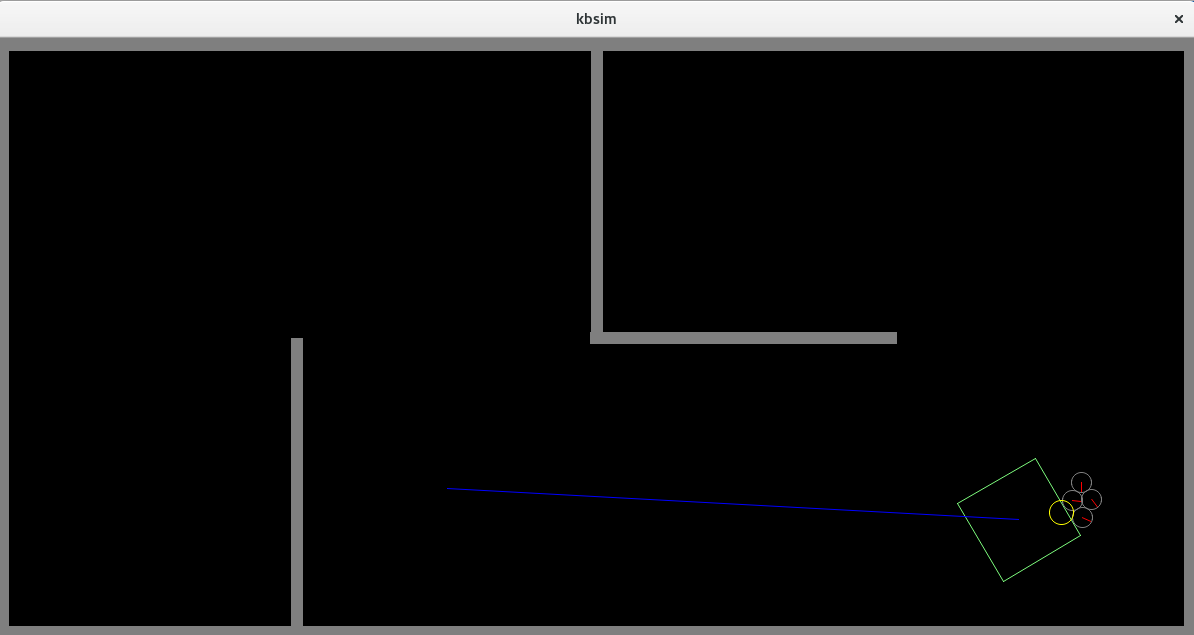
\includegraphics[width=0.9\linewidth]{figures/simulator_maze.png}
    \caption{Simulator showing 4 kilobots pushing an object through a maze}
    \label{fig:simulator}
\end{figure}

\subsection{Object Movement Policy}
\label{sec:objpolicy}


% sample generation iteration
% states
% features

\section{RESULTS}

\section{FUTURE WORK \& CONCLUSION}


\bibliographystyle{plainnat}
\bibliography{bibliography}

\end{document}
